%
% Modified by Sameer Vijay
% Last Change: Wed Jul 27 2005 13:00 CEST
%
%%%%%%%%%%%%%%%%%%%%%%%%%%%%%%%%%%%%%%%%%%%%%%%%%%%%%%%%%%%%%%%%%%%%%%%%
%
% Sample Notre Dame Thesis/Dissertation
% Using Donald Peterson's ndthesis classfile
%
% Written by Jeff Squyres and Don Peterson
%
% Provided by the Information Technology Committee of
%   the Graduate Student Union
%   http://www.gsu.nd.edu/
%
% Nothing in this document is serious except the format.  :-)
%
% If you have any suggestions, comments, questions, please send e-mail
% to: ndthesis@gsu.nd.edu
%
%%%%%%%%%%%%%%%%%%%%%%%%%%%%%%%%%%%%%%%%%%%%%%%%%%%%%%%%%%%%%%%%%%%%%%%%

%
% Chapter 3
%

\chapter{TWO PROTON TRANSFER AT NOTRE DAME}
\label{chap:2pExpt}

Give an overview of the requirements for two-proton transfer and say that ND has a buncher and a Tandem accelerator that goes up to 10 MV so we can get beam energies up to 20 MeV for 3He and we have a beamline with a long flight path SO we can do this experiment.

The previous chapter demonstrated the interest in studying the (3He,n) transfer reaction onto 76Ge; this chapter will discuss the beam and detector properties that are necessary for measuring the angular distribution of this reaction.

One obvious requirement is 3He beam.  The Helium Ion Source (HIS) at Notre Dame can produce microamps of Helium beam; He gas is provided to the ion source.  To make 3He beam, 3He gas must be provided to the ion source.  While in principle this is not difficult, in practice 3He gas is prohibitively expensive.  

Another consideration is the beam energy.  Because the reaction of interest is a nuclear reaction, the energy must be above the Coulomb barrier.  To maximize the cross section, the beam energy must be near 18 MeV.

The Tandem Van deGraff at Notre Dame has a maximum terminal voltage of 10 MV.  Beam from the HIS is singly, negatively ionized.  The beam stays in this ionization state until it encounters a carbon foil in the center of the accelerator terminal and is stripped of all its electrons, leaving it 3He2+.  In the case of 3He beam, then, the energy of the accelerated beam is 

E = 3V

where V is the terminal voltage.

For an 18 MeV 3He beam, the terminal voltage required is 6 MV, easily provided by the Tandem Accelerator.

So far, then, the facility at Notre Dame can easily supply the necessary beam at the ideal energy.  But neutron detection imposes an additional constraint on the beam.

The resulting products of a two-proton transfer onto 76Ge are a neutron and a 78Se nucleus.  Our detector has poor neutron detection efficiency, but the heavy, charged 78Se nucleus is unlikely to escape the target, forcing us to rely on neutron detection to study this reaction.  

Imagine for a moment the options that are available to the neutron that wishes to interact with any detector.  It has no charge, so disturbing electrons via the electromagnetic force is not possible.  The neutron can interact with the electrons weakly, but this probability is impractically small.  A neutron may also interact with a proton, strongly.  This strong interaction is predominantly responsible for neutron detection.  A neutron that transfers some of its energy to a proton can rely on the proton, in all its charged glory, to register a signal in the detector.  What experimenters must do is provide plenty of protons for neutrons to collide with - large quantities of water or plastics, with their long hydrocarbon chains, are popular choices.

What does a neutron signal look like in such a detector?  If the neutron always deposited all its energy in the detector, the energy spectrum would show sharp peaks corresponding to each neutron energy.  Sadly, a neutron interacting with a proton rarely transfers all its energy to that proton.  In this transfer experiment, it is necessary to identify signals coming from neutrons - worse, specific neutrons!  The neutrons of interest are those coming from the ground state of the daughter nucleus, not neutrons from its many excited states.  Because the neutron's deposited energy does not determine that neutron's full energy, the experiment must be sensitive to some quantity that gives unambiguous information about the neutron's energy.

% figure of charged-particle energy spectrum
% figure of neutron energy spectrum

Time is uniquely determined by the neutron's energy - the time it takes for the neutron to travel from the target to the detector depends on its energy as in \eq \ref{eq:TOF}.  

\begin{equation}
\frac{v}{c} = \sqrt{\frac{E^2 - m^2c^4}{E^2}}
\label{eq:TOF}
\end{equation}

Measuring the time of flight (TOF) of the neutron to sufficient accuracy requires both beam bunching and a long neutron flight path.  In a continuous beam, there is no way to know which 3He was associated with a neutron event in the detector, and therefore no way to determine TOF.  Bunching the beam so that clumps of 3He arrive at the same time and providing a signal correlated to their arrival at the target allows a TOF measurement with a precision determined by the time-width of the bunch.  This limit on time resolution constrains the distance between the target and detector.  In this experiment, it is necessary to distinguish between neutrons whose energies differ by only 0.5 MeV.  With a flight path of 1 m between the target and detector, the difference in time between these two neutrons is ?? ns - far less than the resolution determined by the beam bunch.  The flight path must be long enough to distinguish ground state neutrons from neutrons associated with the first excited state of the residual nucleus.

\section{Beam Production at Notre Dame}
The beam delivered to the target is ?? MeV bunched 3He.  In this section, we will follow the beam through its production and accelaration.

The accelerator at Notre Dame is a Van deGraff accelerator made by High Voltage Engineering.  Its maximum potential is 10 MV and is a tandem Van deGraff - a thin Carbon target in the center of the machine strips electrons, providing additional acceleration to the beam.  The ion source must provide negatively charged ions to the Tandem's first acceleration stage.

The Helium Ion Source, made by ??, provides negative 3He ions by adding electrons to 3He gas.  A chamber filled with 3He gas converts some of the gas into plasma with a filament that discharges to the chamber wall.  Electrostatic elements extract the plasma into a region filled with Cesium vapor.  Because Cesium donates electrons generously, some 3He becomes ionized and will follow the electric potential into the switching magnet.  A dipole magnet is necessary after the ion source because the carbon, oxygen, and other impurities contaminate the 3He beam.  Movable, thick tungsten slits allow only beam in a small range of rigidity through to the Tandem accelerator.

Accelerated beam leaving the Tandem encounters a large dipole magnet that selects beam of the desired energy.  This magnet is tuned using the NMR frequency of Hydrogen (?) and has an error of less than ?? (units?).  Comparing this energy spread to the energy spread introduced by the target gives a sense of how small the error associated with the beam energy is; the target spreads the energy by 0.5 MeV.

\subsection{Beam Focusing}

The accelerated beam must travel from the accelerator to a target ?? m through four inch beampipe; many focusing and steering elements are necessary for a reasonable transmission rate.  Two Einzel Lenses focus the beam before it enters the accelerator, and a set of electrostatic steerers before and after the accelerator are enough to position the beam before it enters the energy-selecting dipole magnet.

Quadrupole triplet and doublet magnets focus the beam as it travels through the target rooms, and another set of electrostatic steerers allows correction of the beam angle.  The final focusing element before the target are two large-bore, variable-strength solenoid magnets that focus the beam to a spot approximately 2 mm in diameter.

% figure: beamline

\subsection{Beam Bunching}
Discuss the operation of the buncher, pulse selector, and sweeper.  Discuss beam loss, which actually isn't too bad since we're radiation-limited in the target room.
Time resolution ~ 1ns which again isn't too bad since our detector has similar resolution.
Discuss modifications made to buncher platform?

Continuous beam would make it impossibile for our detectors to distinguish between beam-related neutron events and gamma events.  It is possible to bunch the beam so that ``bunches'' of 3He arrive at the target, each bunch having a time spread of less than one ns.  

The beam buncher at Notre Dame works by slowing down particles that would arrive too early at the target and speeding up particles that would be arriving too late.  To acheive this, two grids perpendicular to the beam connect to a power supply create an electric field that varies in time.  Bunching all the beam requires that the electric field be a triangle wave in time, but commercially available power supplies providing adequate current and rapid enough signal generally vary sinusoidally in time.  At some beam facilities \cite{LynchBunching}, multiple power supplies provide additional frequncies, better approximating a triangle wave.  At Notre Dame, one frequency, 11 MHz, is used.  The best bunching occurs when the wave is at its steepest; when the electric field is changing very slowly, little bunching occurs.  The effect of the bunching, then, is that the beam is continuous, with large bunches every 101 ns.  The beam in between these bunches would render our time signal useless, and must somehow be removed.

The ``sweeper'' provides a large electric field that ramps up and down very quickly to remove the unwanted beam between the bunches.  While conceptually simple, the time scale required for the charging of the plates makes it difficult to find a commercially available power supply.  The field must turn ``on'' on a timescale much smaller than the beam bunch, or else become the limiting factor in the time-width of the bunch.  The power supply used provides ?? charge in ?? ns.

%figure of beam profile and sweeper

The beam buncher and sweeper are all that is needed to provide bunched beam.  At Notre Dame, the beam bunches are 101.52 ns apart and are typically 1 ns to 2 ns wide.  This bunch spacing presents a problem for the experiment because the neutron TOF is in excess of 200 ns.  With bunches arriving at the target every 100 ns, it will be impossible to tell if a neutron is very slow and associated with bunch A or very fast and associated with bunch B.  The spectrum will be considerably complicated.

% figure: the considerably complicated spectrum

To give all the neutrons resulting from one beam bunch time to reach the detector before the next bunch strikes, a ``pulse selector'' knocks out three of every four bunches, resulting in 300 ns between each bunch.  Even with such generous time between bunches, there are very slow neutrons from previous bunches that overlap with gammas from the current bunch, but these vanish with even a low energy cut.

% figure: slow neutrons and their dissappearance

Beam bunching dramatically reduces available beam - swept beam current is ?? less than its non-bunched.  But without bunched beam it would not be possible to distinguish the neutrons of interest in the (3He,n) transfer reaction.  Despite this limited current, the Notre Dame facility cannot improve the statistics of this experiment beyond a factor of ?? because the radiation limits on the room with the detector are so low that even with pulse selection, the beam is near its maximum allowed current.


\section{The Neutron Detector}
Discuss neutron wall briefly.  Can reference NIMA paper. Explain why it's important that it's wide-angle. 
Electronics diagram!  Discuss two most important aspects: TDC and ADC from phototubes

The neutron detectors are large strips of high density polyethylene (HDPE) plastic doped with scintillator (what kind of scintillator??).  Sixteen independent detectors sit in a rough circle around the target, with the forwardmost angle being 5$\circ$ and the largest angle being $21\circ$.  The angle step size between each detector is approximately 0.7$\circ$.  The detectors sit 15.6 m away from the target to ensure a resolution of at least 0.5 MeV at 22 MeV.  This distance comes at a steep price; the solid angle is only (approx. 10 cm/15 m x 2.5 m/15 m = 0.11) sr, or 0.88\% of the unit circle.

% figure - picture of detector

The plastic scintillator, equipped with fast timing PMT's, are sensitive to energy deposition and time.  Energy deposited is not useful for neutron identification; it is timing information that ID's neutrons.  In principle, the timing information is all the DAQ needs to record.  This would be true if only there were no background radiation!  The low-energy gamma radiation from the concrete leaves signal in the detector at a high rate - much higher than the rate of beam! Measuring the Energy deposition is crucial because it allows us to throw out low-energy background from the room.  

What is clear is that while energy information is necessary, the energy information does not need to be terribly precise.  The timing information, however, must be as precise as possible.  The goal for the electronics is to not add spread to the timing that is noticable above the timing spread already inherent in the beam bunching.  The detectors are equipped with photomultiplier tubes (PMT's) at the top and bottom that have excellent timing response - their risetime is approximately 5 ns.  Constant Fraction Discriminators (CFD's) give timing information with jitter that's less than 1 ns.

\subsection{Electronics}
When a real event occurs in some bar of the neutron detector, the DAQ must record the energy and time of both the top and bottom PMT of that bar.  A QDC can integrate the PMT signal and a TDC can measure the time between a logic pulse created by the PMT signal and the logic pulse from the beam buncher.  Because time resolution is crucial, constant fraction discriminators (CFD's) and not leading edge discriminators create the logic pulse sent to the TDC.  

The lone signal provided by the PMT base is not adequate for this processing because two signals, one for the QDC and one for the TDC, are necessary.  The signal from the PMT base is also too small to trigger the CFD's.  The ?? x10 amplifier makes the signal large enough to trigger the CFD's and provides two copies of the input signal, one which can be analyzed for timing information while the other is analyzed for energy information.  A diagram of the data acquisition concept is shown in fig ??.

% figure: simple electronics
\begin{figure}[ht]
\centering
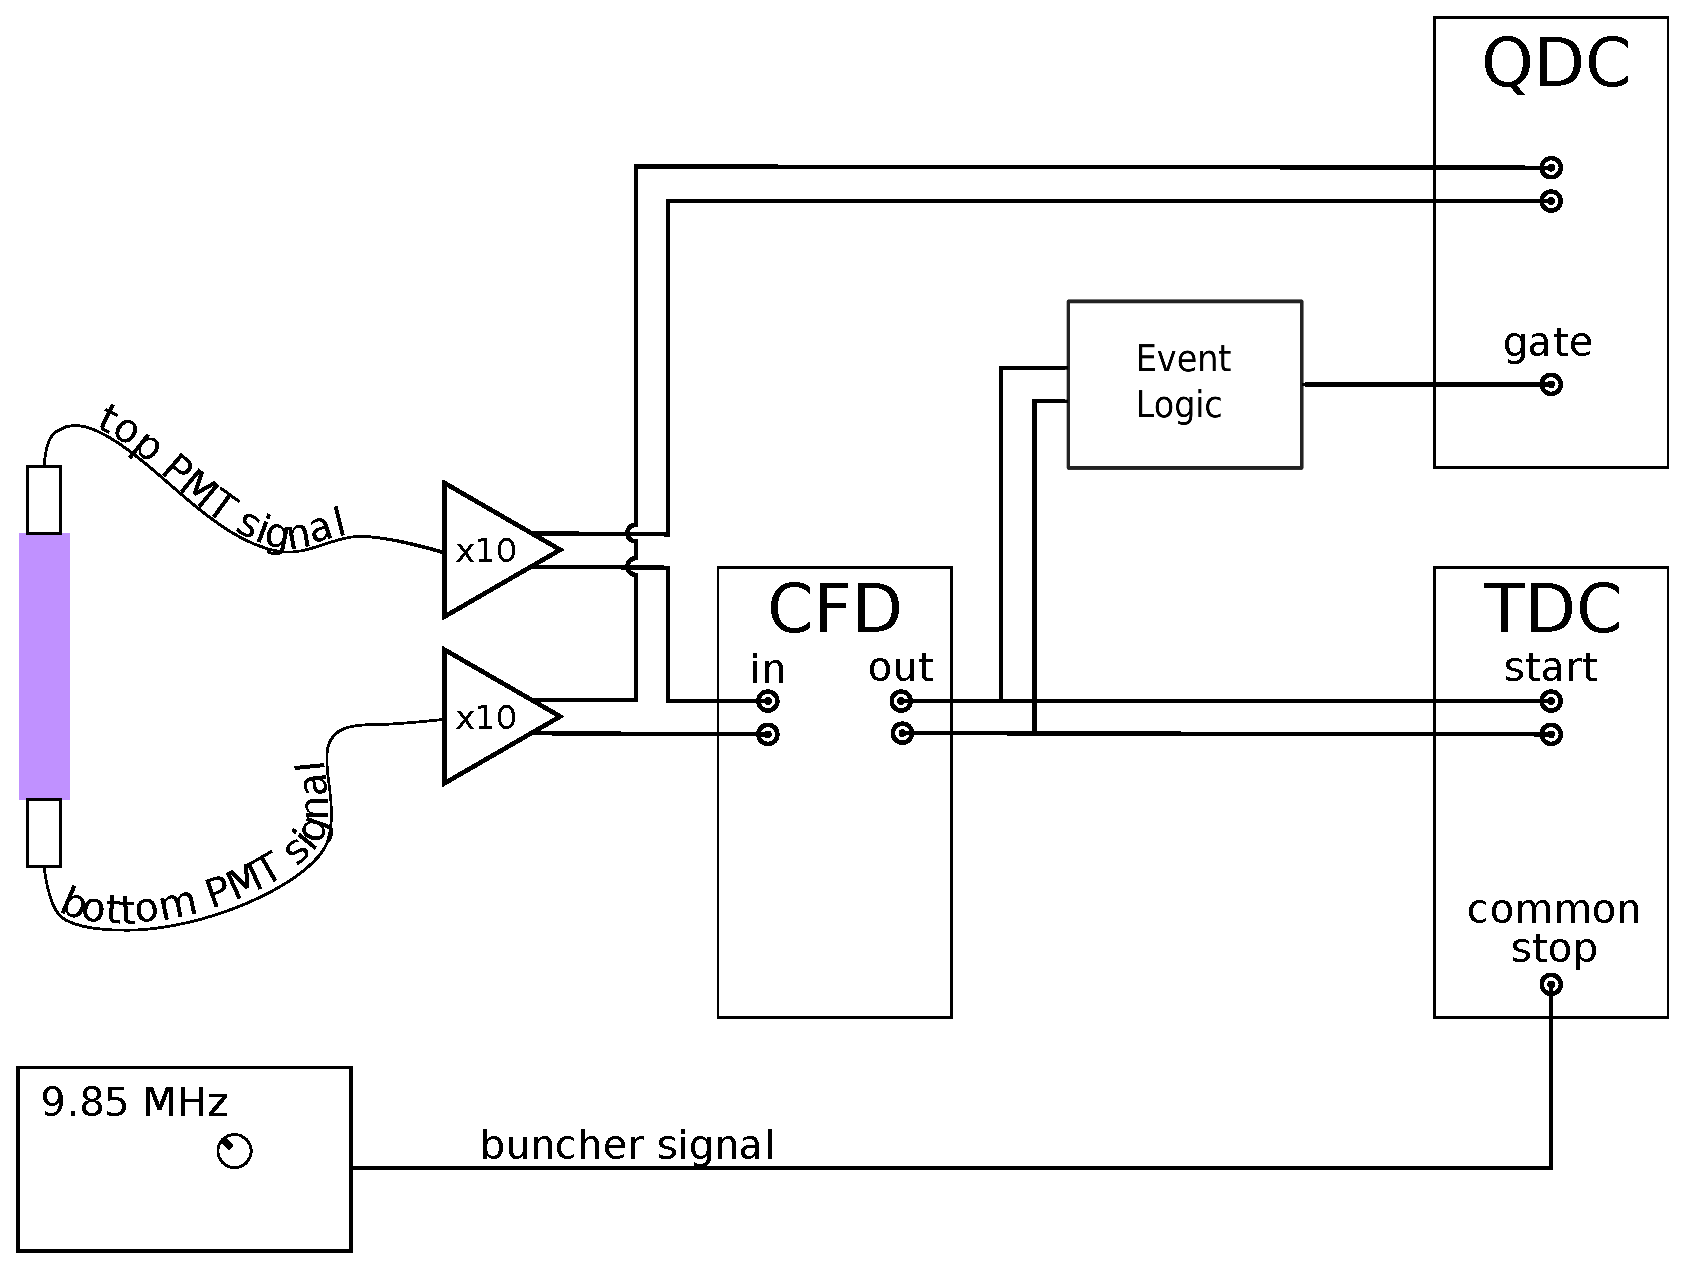
\includegraphics[width=1.0\textwidth]{figures/basic_electronics.eps}
\label{fig:simpleElectronics}
\caption{A simplified diagram of the neutron detector electronics showing the acquisition of timing and energy information from the detectors.}
\end{figure}

What is a good trigger to construct for the neutron wall?  For just one neutron detector, triggering any time the top or bottom PMT fired would waste the DAQ with recording many noise events.  A real event should result in signal in both the top and bottom PMT's, and requiring a coincidence between the two results in a reasonable trigger.  One way to define an event trigger for the entire neutron wall, then, would be to trigger any time a coincidence between associated top and bottom PMT's occurs.  But constructing this trigger with NIM logic units requires 16 separate logic gates and would require purchasing additional, expensive logic modules.  

The solution is to use the built-in 'OR' of the CFD.  Instead of requiring a top and bottom signal in the same bar, the condition is loosened to requiring a signal in a top PMT and a bottom PMT in the same eight-bar group.  Each CFD is an eight-fold unit and provides an 'OR' output.  Each CFD receives only top or bottom signals.  The presence of some top signal AND some bottom signal triggers the event signal.  Such an event only knows that both a top and bottom signal coincided but is blind to whether or not these signals belonged to the same bar.  Such an event trigger includes all events where the top and bottom signal belong to one bar but also includes spurious events where no bar has signal in both its top and bottom PMT.  With a dead time of less than 30\%, this event condition does not hinder data collection, and simple software cuts eliminate spurious events.

% figure: event trigger
\begin{figure}[ht]
\centering
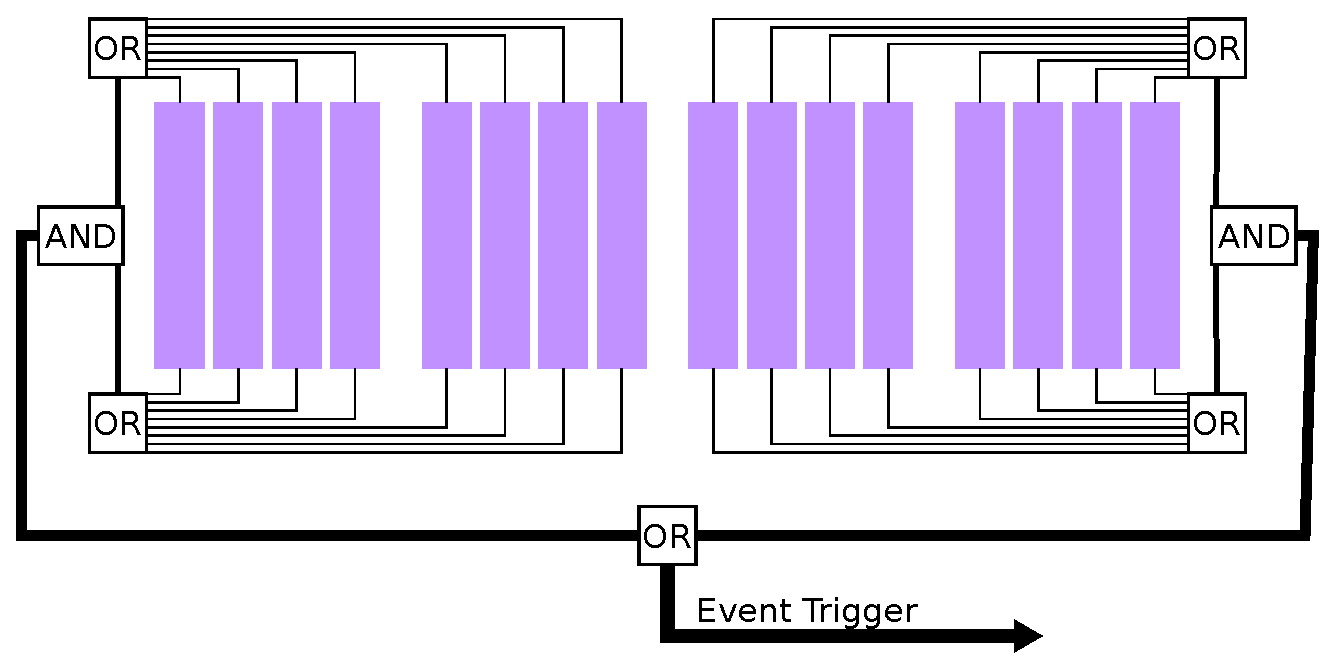
\includegraphics[width=1.0\textwidth]{figures/event_trigger.eps}
\label{fig:eventTrig}
\caption{The event trigger for the DAQ requires a coincidence between a top PMT and a bottom PMT from the same group of eight detectors.}
\end{figure}


\section{Setup}
Flight path and time resolution as a function of neutron energy - apply this to Ge ground and first excited state!
Beam monitor
Dead time
Include a sample calculation?  Like: this is what we see in the detector.  To get an absolute cross-section, here is the calculation:
counts * time * particle current * target thickness
So we get the counts this way and the time with the signal from the DAQ and the target thickness from Hope



\subsection{Testing with 26Mg}
Show results from first run and look at timing - hey it's all right!
Look at background - will need to improve

% % uncomment the following lines,
% if using chapter-wise bibliography
%
% \bibliographystyle{ndnatbib}
% \bibliography{example}
